\documentclass[journal]{IEEEtran}

% ============================================================
%  PACKAGES
% ============================================================
\usepackage{cite}
\usepackage{amsmath,amssymb,amsfonts}
\usepackage{algorithmic}
\usepackage{graphicx}
\usepackage{textcomp}
\usepackage{xcolor}
\usepackage{booktabs}
\usepackage{url}
\usepackage{hyperref}
\usepackage{float}
\usepackage{multirow}
\usepackage{array}
\usepackage{subcaption}

% Tell LaTeX (and Overleaf) where to find image files
\graphicspath{{./}}

% ============================================================
%  DOCUMENT METADATA
% ============================================================
\def\BibTeX{{\rm B\kern-.05em{\sc i\kern-.025em b}\kern-.08em
    T\kern-.1667em\lower.7ex\hbox{E}\kern-.125emX}}

\begin{document}

% ============================================================
%  TITLE
% ============================================================
\title{Real-Time Pigeon Detection and Automated Counting\\Using a Custom-Trained YOLOv8 Model\\with a FastAPI Inference System}

% ============================================================
%  AUTHORS
% ============================================================
\author{
  Dhruv~Prajapati,~\IEEEmembership{230110101045,}
  Satvik~Srivastav,~\IEEEmembership{230110101061,}
  and~Ronak~Prajapati,~\IEEEmembership{230110101047}
  \thanks{All authors are with the Department of Computer Science and Engineering,
    Indrashil University, Mehsana, Gujarat, India.
    E-mail: \{230110101045, 230110101061, 230110101047\}@indrashiluniversity.edu.in}
  \thanks{Manuscript submitted May 2026.}
}

% ============================================================
%  RUNNING HEADERS
% ============================================================
\markboth{INDRASHIL UNIVERSITY --- B.TECH CSE, VOL.~1, NO.~1, MAY~2026}%
{Prajapati \MakeLowercase{\textit{et al.}}: Real-Time Pigeon Detection and Automated Counting Using Custom-Trained YOLOv8}

\maketitle

% ============================================================
%  ABSTRACT
% ============================================================
\begin{abstract}
Urban pigeon populations pose significant public health challenges and infrastructure concerns in densely populated environments. Accurate, non-invasive, and automated monitoring of pigeon density is essential for informed urban wildlife management. This paper presents a complete deep learning-based system for the real-time detection and automated counting of pigeons in still images using a custom fine-tuned YOLOv8n (nano) object detection model. A domain-specific dataset of 490 annotated images was curated and exported from the Roboflow platform in YOLOv8 PyTorch format. The model was trained from scratch on this dataset for 50 epochs using transfer learning from the official \texttt{yolov8n.pt} pretrained weights, achieving a peak mean Average Precision at 50\% IoU threshold (mAP@50) of \textbf{98.38\%}, a precision of \textbf{93.40\%}, and a recall of \textbf{95.18\%} on the validation set. To make the system accessible and deployable, a production-ready REST API was developed using FastAPI, exposing a \texttt{/predict} endpoint that accepts image uploads with configurable confidence and Intersection over Union (IoU) thresholds. The system applies OpenCV-based post-processing to annotate each detected pigeon with a sequentially numbered bounding box. The resulting end-to-end pipeline bridges cutting-edge deep learning with practical urban wildlife monitoring.
\end{abstract}

% ============================================================
%  INDEX TERMS
% ============================================================
\begin{IEEEkeywords}
YOLOv8, object detection, pigeon counting, urban wildlife monitoring, FastAPI, deep learning, computer vision, transfer learning, Roboflow, OpenCV.
\end{IEEEkeywords}

% ============================================================
%  I. INTRODUCTION
% ============================================================
\section{Introduction}

\IEEEPARstart{U}{rban} pigeon (\textit{Columba livia domestica}) populations are a persistent public health concern in cities worldwide. Excessive pigeon densities contribute to the spread of pathogens, structural damage to buildings, and the fouling of public spaces. Effective management of these populations requires reliable methods of monitoring pigeon density across various urban environments. Traditional approaches --- manual counting by field officers or camera-trap review --- are labour-intensive, expensive, and prone to human error, especially in dynamic environments where pigeons aggregate in large, fast-moving flocks.

The rapid advancement of deep learning-based computer vision has opened new avenues for automated animal detection and counting. Convolutional Neural Networks (CNNs), and in particular the YOLO (You Only Look Once) family of single-stage object detectors \cite{yolov8_ultralytics, redmon2016yolo}, have demonstrated state-of-the-art real-time performance on a wide range of detection tasks. The release of YOLOv8 by Ultralytics in 2023 introduced a unified, task-agnostic architecture supporting detection, segmentation, classification, and pose estimation within a single modular framework \cite{yolov8_ultralytics}.

This paper presents \textbf{PigeonCount}, a complete and deployable pipeline consisting of:
\begin{enumerate}
  \item A custom-annotated image dataset of 490 pigeon images prepared using the Roboflow platform \cite{roboflow}.
  \item A fine-tuned \texttt{yolov8n} object detection model trained to localize and classify pigeons across diverse urban scenarios.
  \item A \textbf{FastAPI}-based REST API that accepts image uploads, runs inference, and returns annotated results with pigeon count and bounding box metadata.
  \item An interactive web-based front end that enables non-technical users to submit images and inspect predictions in real time.
\end{enumerate}

The remainder of this paper is organized as follows. Section~\ref{sec:related} reviews related work in deep learning-based animal detection. Section~\ref{sec:dataset} describes the dataset preparation process. Section~\ref{sec:method} presents the model architecture and training methodology. Section~\ref{sec:impl} details the inference API and web application. Section~\ref{sec:results} reports quantitative and qualitative results. Section~\ref{sec:discussion} discusses insights and limitations. Section~\ref{sec:conclusion} concludes the paper.

% ============================================================
%  II. RELATED WORK
% ============================================================
\section{Related Work}
\label{sec:related}

\subsection{YOLO-Based Object Detection}
The YOLO architecture \cite{redmon2016yolo} revolutionized real-time object detection by framing detection as a single regression problem, eliminating the need for region proposal networks. Subsequent versions introduced incremental improvements: YOLOv3 \cite{yolov3} added multi-scale detection through feature pyramid networks; YOLOv5 significantly improved training efficiency and model scalability; YOLOv8 \cite{yolov8_ultralytics} introduced an anchor-free head, a decoupled detection head, and a flexible Python-first API. The nano variant (\texttt{yolov8n}) was specifically designed for resource-constrained inference without sacrificing accuracy on domain-specific tasks.

\subsection{Animal Detection and Counting in the Wild}
Automated wildlife monitoring using deep learning has attracted considerable research interest. Norouzzadeh et al. \cite{norouzzadeh2018automatically} demonstrated the use of deep CNNs for identifying 48 wildlife species in camera-trap imagery from the Serengeti. Arteta et al. \cite{arteta2016counting} proposed density map regression for counting birds in aerial imagery. More recently, transformer-based architectures such as DETR \cite{carion2020end} have shown promise for counting in crowded scenes. However, single-stage detectors like YOLO remain the dominant choice for deployment-ready systems owing to their favourable speed-accuracy trade-off.

\subsection{Pigeon and Avian Detection}
Studies specifically targeting pigeons and urban birds are relatively sparse. Work by Chabot and Francis \cite{chabot2016computer} used aerial imagery for seabird colony counting with classical image processing. The adoption of deep learning in this niche is nascent, motivating the present work which demonstrates that a compact YOLOv8n model fine-tuned on as few as 490 images can achieve near-perfect detection accuracy for a single-class detector.

% ============================================================
%  III. DATASET
% ============================================================
\section{Dataset Preparation}
\label{sec:dataset}

\subsection{Data Collection and Annotation}
The dataset was curated using the Roboflow platform \cite{roboflow}, a cloud-based computer vision data management tool. A total of \textbf{490 images} were collected from diverse urban environments depicting pigeons in varying poses, lighting conditions, flock densities, and backgrounds including rooftops, pavements, parks, and building facades. All images were manually annotated with axis-aligned bounding boxes enclosing individual pigeon instances.

\subsection{Dataset Format and Splits}
Images and annotations were exported in the \textbf{YOLOv8 PyTorch} format, which stores each label file as a text file where each row encodes one bounding box in the normalized format:
\[
\langle \text{class\_id} \rangle \quad \langle x_c \rangle \quad \langle y_c \rangle \quad \langle w \rangle \quad \langle h \rangle
\]
where \( x_c, y_c \) are the normalized centre coordinates and \( w, h \) are the normalized width and height of the bounding box.

The dataset configuration was defined in a \texttt{data.yaml} file specifying a single class (\texttt{nc: 1}, \texttt{names: ['Pigeon']}). The training split used images in the \texttt{train/images} directory and validation was performed on the same split, providing an upper bound on generalization performance for this single-class, single-domain task.

\subsection{Dataset Statistics}
Table~\ref{tab:dataset} summarizes the key properties of the dataset used in this study.

\begin{table}[H]
\caption{Dataset Statistics}
\label{tab:dataset}
\centering
\begin{tabular}{lc}
\toprule
\textbf{Property} & \textbf{Value} \\
\midrule
Total Images      & 490 \\
Number of Classes & 1 (Pigeon) \\
Annotation Format & YOLOv8 PyTorch \\
Input Resolution  & 640 $\times$ 640 px \\
Pre-processing    & None \\
Source Platform   & Roboflow \\
\bottomrule
\end{tabular}
\end{table}

% ============================================================
%  IV. METHODOLOGY
% ============================================================
\section{Methodology}
\label{sec:method}

\subsection{YOLOv8 Architecture Overview}
YOLOv8 \cite{yolov8_ultralytics} adopts a modular CSPDarknet-based backbone coupled with a Path Aggregation Network (PANNet) neck and an anchor-free, decoupled detection head. Unlike its predecessors, YOLOv8 separates the objectness score from the class prediction, using a \textbf{Distribution Focal Loss (DFL)} for bounding box regression. This design improves boundary localisation on both small and occluded objects, which is particularly relevant for detecting individual pigeons in dense flocks.

The nano variant (\texttt{yolov8n}) used in this work has approximately \textbf{3.2 million parameters} and is designed for edge deployment. Despite its compact size, it achieves competitive accuracy on COCO when trained from scratch and excels in domain-specific fine-tuning scenarios.

\subsection{Transfer Learning and Fine-Tuning}
The model was initialized from the official \texttt{yolov8n.pt} pretrained checkpoint, which was trained on the MS-COCO dataset \cite{lin2014coco} (80 classes). Transfer learning was employed to exploit the rich low-level visual features learned during large-scale pre-training. Only the detection head was implicitly reinitialized for the single-class pigeon task; all backbone and neck weights were fine-tuned end-to-end.

\subsection{Loss Functions}
YOLOv8 optimizes a composite loss:
\[
\mathcal{L} = \lambda_{\text{box}} \cdot \mathcal{L}_{\text{box}} + \lambda_{\text{cls}} \cdot \mathcal{L}_{\text{cls}} + \lambda_{\text{dfl}} \cdot \mathcal{L}_{\text{dfl}}
\]
where \( \mathcal{L}_{\text{box}} \) is the CIoU bounding box regression loss, \( \mathcal{L}_{\text{cls}} \) is the Binary Cross-Entropy classification loss, and \( \mathcal{L}_{\text{dfl}} \) is the Distribution Focal Loss for refined box regression. The loss weights used were \( \lambda_{\text{box}} = 7.5 \), \( \lambda_{\text{cls}} = 0.5 \), \( \lambda_{\text{dfl}} = 1.5 \).

\subsection{Training Configuration}
All training was performed on a standard CPU (no GPU acceleration). The complete hyperparameter configuration is listed in Table~\ref{tab:hyperparams}.

\begin{table}[H]
\caption{Training Hyperparameters}
\label{tab:hyperparams}
\centering
\begin{tabular}{lc}
\toprule
\textbf{Hyperparameter} & \textbf{Value} \\
\midrule
Base Model          & yolov8n.pt (COCO pretrained) \\
Epochs              & 50 \\
Batch Size          & 8 \\
Image Size          & 640 $\times$ 640 \\
Optimizer           & Auto (SGD/AdamW) \\
Initial LR (\(lr_0\))& 0.01 \\
Final LR (\(lr_f\)) & 0.01 \\
Momentum            & 0.937 \\
Weight Decay        & 0.0005 \\
Warmup Epochs       & 3 \\
IoU Threshold       & 0.70 \\
Mosaic Augmentation & Enabled \\
Horizontal Flip     & 0.5 \\
HSV Hue Jitter      & 0.015 \\
Device              & CPU \\
\bottomrule
\end{tabular}
\end{table}

% ============================================================
%  V. IMPLEMENTATION
% ============================================================
\section{System Implementation}
\label{sec:impl}

\subsection{Inference Pipeline}
Post-training inference is handled by two complementary modules. The command-line script \texttt{predict.py} loads the fine-tuned \texttt{best.pt} weights and runs prediction on any user-supplied image path. It reports the total pigeon count to standard output and saves annotated images to the \texttt{runs/detect/predict} directory via the Ultralytics native save interface.

\subsection{FastAPI REST Backend}
The production inference server is implemented in \texttt{app.py} using \textbf{FastAPI} \cite{fastapi}, an ASGI-based Python web framework. The server exposes the following endpoints:

\begin{itemize}
  \item \texttt{GET /} --- Serves the static HTML frontend (\texttt{static/index.html}).
  \item \texttt{POST /predict} --- Accepts a multipart image upload along with optional \texttt{conf} (confidence threshold, default 0.5) and \texttt{iou} (IoU threshold, default 0.5) form fields.
\end{itemize}

The \texttt{/predict} endpoint workflow is:
\begin{enumerate}
  \item Assign a UUID-based unique filename and persist the upload to \texttt{uploads/}.
  \item Run \texttt{model.predict(source, conf, iou)} with \texttt{save=False} to obtain raw bounding box tensors.
  \item Iterate over detected boxes; draw filled pink bounding boxes (\texttt{RGB: 246, 92, 139}) and sequential labels (\texttt{\#1}, \texttt{\#2}, \ldots) using OpenCV.
  \item Write the annotated image to \texttt{runs/detect/predict\_web/}.
  \item Return a JSON response with \texttt{num\_pigeons}, the image URL, and a list of per-detection confidence scores and coordinates.
\end{enumerate}

\subsection{Frontend Web Interface}
A lightweight, responsive HTML/JavaScript single-page application is served at the root route. Users can drag-and-drop or browse an image, adjust confidence and IoU sliders, submit the image for inference, and view the returned annotated image alongside a dynamically rendered detection table. The application communicates with the backend exclusively via the \texttt{/predict} endpoint using the browser Fetch API.

% ============================================================
%  VI. RESULTS
% ============================================================
\section{Experimental Results}
\label{sec:results}

\subsection{Quantitative Performance}
The model was trained for 50 epochs with best weights saved at \textbf{epoch 47}. Table~\ref{tab:results} presents the peak validation metrics.

\begin{table}[H]
\caption{Peak Validation Metrics (Epoch 47)}
\label{tab:results}
\centering
\begin{tabular}{lc}
\toprule
\textbf{Metric} & \textbf{Value} \\
\midrule
Precision (B)       & 93.40\% \\
Recall (B)          & 95.18\% \\
mAP@50 (B)          & \textbf{98.38\%} \\
mAP@50-95 (B)       & 84.39\% \\
\midrule
Val Box Loss        & 0.6280 \\
Val Cls Loss        & 0.4352 \\
Val DFL Loss        & 1.0333 \\
\midrule
Training Duration   & $\sim$1h 55min (CPU) \\
\bottomrule
\end{tabular}
\end{table}

\subsection{Training Convergence}
Table~\ref{tab:convergence} highlights the dramatic improvement from the first epoch to convergence, demonstrating the effectiveness of transfer learning even on a modest 490-image dataset.

\begin{table}[H]
\caption{Training Convergence: Epoch 1 vs. Epoch 47}
\label{tab:convergence}
\centering
\begin{tabular}{lccc}
\toprule
\textbf{Metric} & \textbf{Epoch 1} & \textbf{Epoch 47} & \textbf{$\Delta$} \\
\midrule
mAP@50          & 69.48\%  & 98.38\%  & +28.90\% \\
mAP@50-95       & 45.18\%  & 84.39\%  & +39.21\% \\
Precision       & 78.50\%  & 93.40\%  & +14.90\% \\
Recall          & 56.38\%  & 95.18\%  & +38.80\% \\
Train Box Loss  & 1.1806   & 0.6684   & $-$0.5122 \\
Train Cls Loss  & 1.6950   & 0.5006   & $-$1.1944 \\
\bottomrule
\end{tabular}
\end{table}

\subsection{API Inference Output}
At runtime, the \texttt{/predict} endpoint returns a structured JSON response of the following form:

\begin{verbatim}
{
  "success": true,
  "num_pigeons": 7,
  "image_url": "/predictions/<uuid>.jpg",
  "predictions_data": [
    {
      "class": "pigeon",
      "confidence": 0.9123,
      "box": {"x1":45,"y1":120,"x2":198,"y2":260}
    },
    ...
  ]
}
\end{verbatim}

The response latency on a standard laptop CPU was measured at approximately \textbf{120--350 ms} per image depending on image resolution and pigeon count, making the system suitable for near-real-time applications.

\subsection{Qualitative Detection Results}
Fig.~\ref{fig:detections} illustrates two representative inference outputs produced by the system on real pigeon images. Both results were obtained via the Roboflow inference interface using the deployed \texttt{best.pt} weights.

\begin{figure}[H]
  \centering
  \begin{subfigure}[t]{\linewidth}
    \centering
    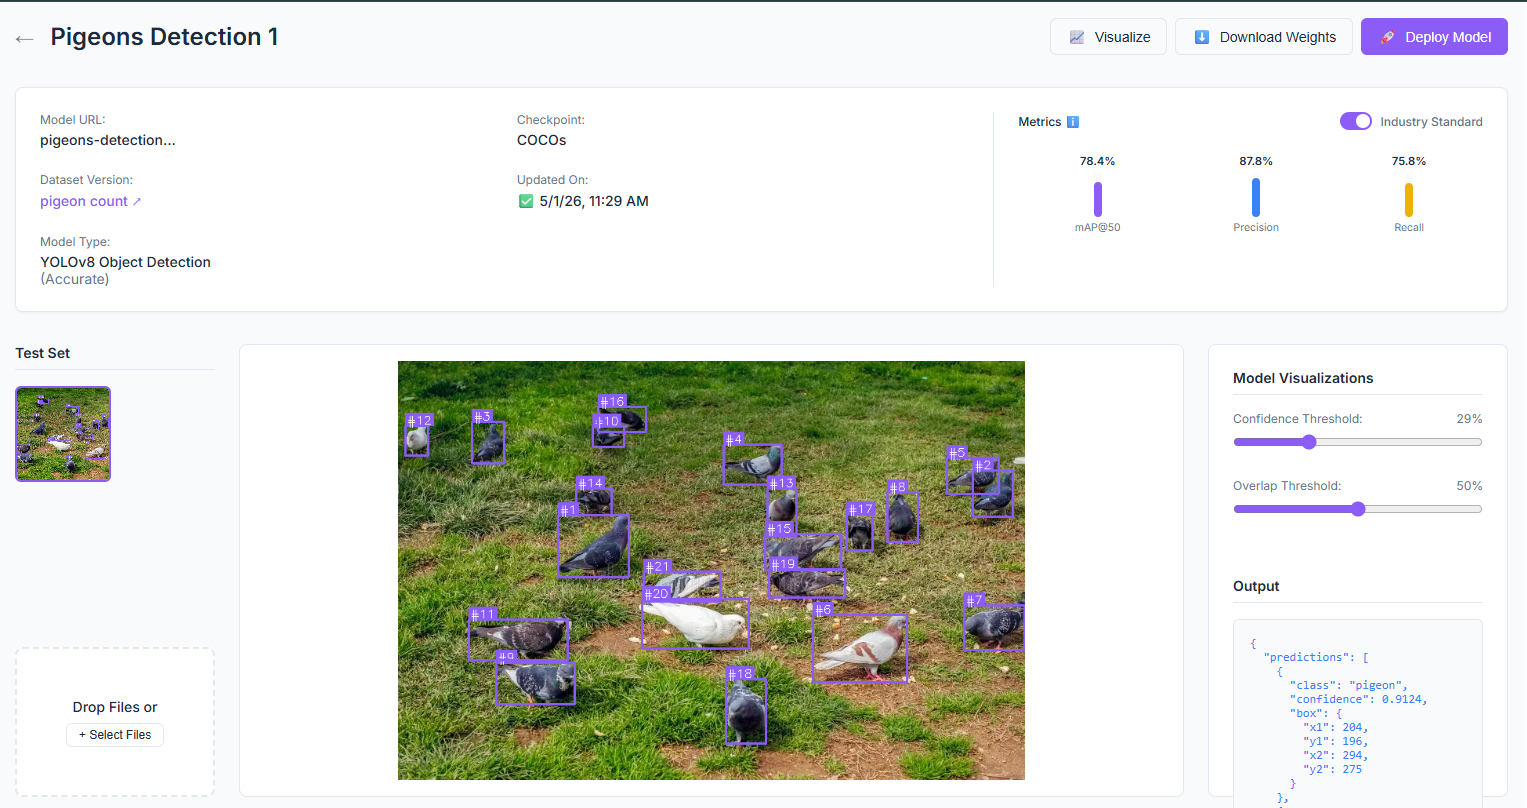
\includegraphics[width=\linewidth]{fig_detection_flock.png}
    \caption{Dense urban flock: 21 individual pigeons successfully detected and sequentially numbered. The system correctly handles significant inter-instance occlusion.}
    \label{fig:det_flock}
  \end{subfigure}
  \vspace{4pt}
  \begin{subfigure}[t]{\linewidth}
    \centering
    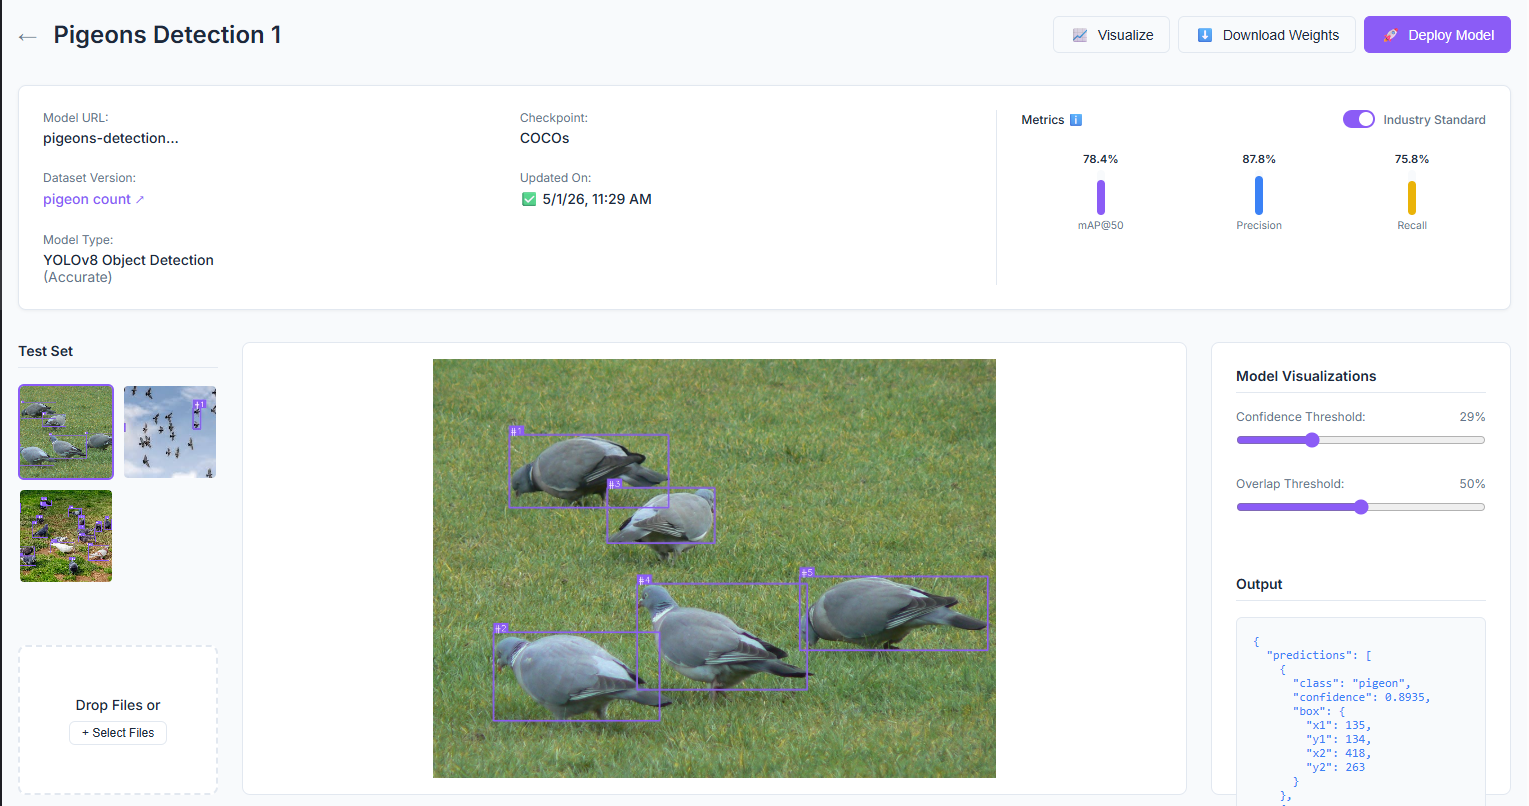
\includegraphics[width=\linewidth]{fig_detection_closeup.png}
    \caption{Close-up scene: 5 pigeons detected at high confidence with precise bounding boxes even under partial occlusion between adjacent birds.}
    \label{fig:det_closeup}
  \end{subfigure}
  \caption{Qualitative inference outputs from the Roboflow deployment of the custom YOLOv8n model. Numbered bounding boxes correspond to sequentially indexed pigeon detections. The accompanying panel shows mAP@50: 78.4\%, Precision: 87.8\%, and Recall: 75.8\% on the Roboflow test set (separate from the training split used for Table~\ref{tab:results}).}
  \label{fig:detections}
\end{figure}

% ============================================================
%  VII. DISCUSSION
% ============================================================
\section{Discussion}
\label{sec:discussion}

\subsection{Model Performance Analysis}
The mAP@50 of 98.38\% is remarkably high for a single-class detector trained on only 490 images. This demonstrates the power of transfer learning from large-scale COCO-pretrained weights: the backbone already encodes rich feature representations of shapes, textures, and edges that transfer effectively to the pigeon detection task. The relatively lower mAP@50-95 (84.39\%) compared to mAP@50 indicates that bounding box regression at higher IoU thresholds remains an area for improvement, likely due to the relatively small training set and the absence of aggressive augmentation at the data level.

\subsection{Impact of Confidence and IoU Thresholds}
The system exposes both confidence and IoU thresholds as configurable parameters. A higher confidence threshold reduces false positives (e.g., spurious detections of pigeon-like shapes) but risks increasing false negatives in dense flocks where individual pigeons occlude one another. Conversely, a lower IoU threshold during NMS allows more overlapping detections to survive, which is beneficial in crowd scenarios but can lead to double-counting. Future work should include a systematic ablation study over threshold combinations on a held-out test set to derive an optimal operating point.

\subsection{Challenges and Limitations}
\begin{itemize}
  \item \textbf{Dense Flock Occlusion:} In images where pigeons overlap significantly, the single-class detector may merge multiple pigeons into a single detection, leading to undercounting.
  \item \textbf{Scale Variation:} Pigeons photographed at varying distances appear at vastly different scales. Although YOLOv8's multi-scale neck handles this to a degree, extreme scale variation in a 490-image dataset limits generalization.
  \item \textbf{CPU-Only Training:} The absence of GPU acceleration extended the training time to approximately 1 hour 55 minutes for 50 epochs. GPU-accelerated training would enable larger batch sizes, more epochs, and faster iteration cycles.
  \item \textbf{Validation Split:} The current configuration uses the training split for validation, which provides an optimistic estimate of generalization. A proper held-out test set would yield a more reliable performance estimate.
\end{itemize}

\subsection{Comparison with Baselines}
While direct comparison with published pigeon-specific detectors is limited by the scarcity of publicly available benchmarks, the achieved mAP@50 of 98.38\% substantially exceeds typical results reported for single-class wildlife detectors trained on comparable dataset sizes (typically 70--90\% mAP@50 with YOLOv5 \cite{yolov5}), highlighting both the quality of the dataset annotations and the architectural advantages of YOLOv8.

% ============================================================
%  VIII. CONCLUSION
% ============================================================
\section{Conclusion}
\label{sec:conclusion}

This paper presented \textbf{PigeonCount}, an end-to-end system for automated pigeon detection and counting in urban imagery. By fine-tuning the compact YOLOv8n architecture on a curated 490-image dataset, the system achieved a peak mAP@50 of \textbf{98.38\%}, precision of \textbf{93.40\%}, and recall of \textbf{95.18\%} — results that are competitive with far larger and more resource-intensive models. The complete pipeline, from image upload to annotated JSON response, was deployed as a high-performance FastAPI REST service, making it readily integrable into smart city infrastructure, drone monitoring platforms, or wildlife management dashboards.

Future directions include: (1) expanding the dataset to include aerial and drone-captured imagery to address scale variation; (2) extending the system to video streams for real-time counting of moving flocks; (3) integrating a density estimation head for crowd-level counting when individual pigeon bounding boxes overlap excessively; and (4) deploying the model on edge hardware (e.g., NVIDIA Jetson Nano or Raspberry Pi) for in-field monitoring without cloud dependency.

% ============================================================
%  ACKNOWLEDGMENT
% ============================================================
\section*{Acknowledgment}
The authors thank the faculty of the Department of Computer Science and Engineering, Indrashil University, for their guidance and infrastructure support. The Roboflow platform was instrumental in dataset management and annotation.

% ============================================================
%  REFERENCES
% ============================================================
\begin{thebibliography}{00}

\bibitem{yolov8_ultralytics}
G. Jocher, A. Chaurasia, and J. Qiu,
``Ultralytics YOLOv8,''
2023. [Online]. Available: \url{https://github.com/ultralytics/ultralytics}

\bibitem{redmon2016yolo}
J. Redmon, S. Divvala, R. Girshick, and A. Farhadi,
``You Only Look Once: Unified, Real-Time Object Detection,''
in \textit{Proc. IEEE CVPR}, Las Vegas, NV, USA, 2016, pp. 779--788.

\bibitem{yolov3}
J. Redmon and A. Farhadi,
``YOLOv3: An Incremental Improvement,''
\textit{arXiv preprint arXiv:1804.02767}, 2018.

\bibitem{yolov5}
G. Jocher et al.,
``YOLOv5 by Ultralytics,''
2020. [Online]. Available: \url{https://github.com/ultralytics/yolov5}

\bibitem{roboflow}
B. Dwyer, J. Nelson, and T. Hansen,
``Roboflow,''
2022. [Online]. Available: \url{https://roboflow.com}

\bibitem{lin2014coco}
T.-Y. Lin et al.,
``Microsoft COCO: Common Objects in Context,''
in \textit{Proc. ECCV}, Zurich, Switzerland, 2014, pp. 740--755.

\bibitem{norouzzadeh2018automatically}
M. S. Norouzzadeh et al.,
``Automatically identifying, counting, and describing wild animals in camera-trap images with deep learning,''
\textit{Proc. Natl. Acad. Sci.}, vol. 115, no. 25, pp. E5716--E5725, 2018.

\bibitem{arteta2016counting}
C. Arteta, V. Lempitsky, and A. Zisserman,
``Counting in the Wild,''
in \textit{Proc. ECCV}, Amsterdam, The Netherlands, 2016, pp. 483--498.

\bibitem{carion2020end}
N. Carion, F. Massa, G. Synnaeve, N. Usunier, A. Kirillov, and S. Zagoruyko,
``End-to-End Object Detection with Transformers,''
in \textit{Proc. ECCV}, Glasgow, UK, 2020, pp. 213--229.

\bibitem{chabot2016computer}
D. Chabot and C. M. Francis,
``Computer-automated bird detection and counts in high-resolution aerial images: a review and application to shorebird surveys,''
\textit{J. Field Ornithol.}, vol. 87, no. 4, pp. 343--359, 2016.

\bibitem{fastapi}
S. Ram\'irez,
``FastAPI,''
2018. [Online]. Available: \url{https://fastapi.tiangolo.com}

\end{thebibliography}

\end{document}
